\chapter{Distributed Hash Table System} \label{Distribution}

This chapter covers designing \DHTS, a distributed hash table system based on the implemented local \PHT.

\section{Overview}

    \DHTS is built on top of a cluster of \Nodes that can run various multithreaded applications. Since \DHTS is a distributed hash table, in our case, each \Node maintains a local \PHT to store a subrange of key-value pairs. \DHTS is symmetrical, with each \Node having the same set of responsibilities as its peers. There is no central coordinator or a supervisor, which makes \DHTS cope well with server crashes.

    \DHTS relies on the consistent hashing method (see Section~\ref{ConsistentHashing}) to distribute data over the cluster. Each key-value pair is replicated on different \Nodes for fault-tolerance. The number of \Nodes which replicate each data item depends on the configuration parameter called the \emph{replication factor}.

    \DHTS provides an interactive administrator console which allows one to manually perform operations on the hash table (\insertMethod, \getMethod, \removeMethod, \iterateMethod), as well as list all known \Nodes and test whether another \Node is connected to the network.
    Naturally, \DHTS features also mechanisms that allowed us to conduct stress tests and the system's performance.

\section{Implementation details}
    \subsection{Decentralised and symmetrical network}
        In a centralised system implementing a hash table, the coordinator is responsible for distributing data between the nodes. In such an approach the nodes' role reduces to performing simple hash table operations on their local fragments of the distributed hash table. However, in such an implementation the crash of the master node causes the entire system to malfunction.
        
        To provide robust fault-tolerance, we decided to implement \DHTS in a decentralised manner, what heavily influences the application design.
    
        Decentralisation implies that no single master node controls the data flow in the system. This requires the nodes to be autonomous and distribute the data themselves.
        To facilitate this, the \Nodes in \DHTS utilise a shared \texttt{hash} method for hashing both the \Nodes and the hash table entries. This way each \Node is able to independently determine which \Node (or a set of \Nodes) is responsible for a key given.
        
        The requirement of a decentralised design results in a quite a complicated implementation of a \Node. However, it is the only way to achieve high availability and gracefully handle server crashes.

    \subsection{Structure}
        The implemented system is composed of several components.

        In order to easily establish and maintain connections between network participants we provide the \Session class. It is a TCP socket wrapper presented in which implements the following methods (see also Listing~\ref{SessionListing}):
        
        \begin{itemize}
            \item \texttt{connect} -- tries to establish a connection on a socket with a \Node listening on an IP address and port given,
            \item \texttt{read} -- wraps the \texttt{async\_read} method from \Asio with exception handling; it also serves incoming messages,
            \item \texttt{write} -- wraps the \texttt{async\_write} method from \Asio with exception handling,
            \item \texttt{get} -- prepares a get request for a key given and sends it over the socket,
            \item \texttt{insert} -- prepares an insert request for a key given (with the provided data) and sends it over the socket,
            \item \texttt{remove} -- prepares a remove request for a key given and sends it over the socket.
        \end{itemize}

\begin{figure}[ht] 
\renewcommand{\figurename}{Listing}
    \begin{lstlisting}
template <class K, class V>
class Session {
    tcp::socket socket;
    
    public:
        Session(tcp::socket socket);
        void connect(std::string address, std::string port);
        void read();
        void write(std::string message);
        void get(K key);
        void insert(K key, V value);
        void remove(K key);
}
\end{lstlisting}
\caption{The Session class}
\label{SessionListing}
\end{figure}

The core class is called \Node and is presented in Listing~\ref{NodeListing}. It is responsible for spawning threads from the \std namespace, each of which asynchronously accepts connections using the \texttt{accept} method. For every incoming connection, an object of the \Session class is created and added to the pool of the already established sessions. The class uses \texttt{io\_context} object from \Asio library to handle \texttt{epoll} on Linux.

\begin{figure}[ht] 
\renewcommand{\figurename}{Listing}
\begin{lstlisting}
class Node {
    boost::asio::io_context &io_context;
    short port;
    
    public:
        Node(boost::asio::io_context &io_context, short port);
        void start();
        void accept();
        void multicast_insert();
        void multicast_remove();
}
    \end{lstlisting}
\caption{The Node class}
\label{NodeListing}
\end{figure}
        
The \KnownNode class allows a \Node to store all the necessary information about a remote \Node it is already connected to.
Each \KnownNode object consists of its own address and port as well as a pointer to the \Session object associated with the connection between itself and the \Node. 
Additionally, each \KnownNode has a hash value assigned (we later discuss how the hash is computed).

\begin{figure}[ht] 
\renewcommand{\figurename}{Listing}
    \begin{lstlisting}
class KnownNode {
    public:
        std::string addr;
        std::string port;
        Session *_session;
        int32_t hash;
        long timestamp;

        KnownNode(Session *_session, std::string address,
                      std::string port, std::int32_t hash);
}
    \end{lstlisting}
    
\caption{The KnownNode class}
\label{Node}
\end{figure}

        All \texttt{KnownNodes} are stored in a simple hash map called \NodesMap. To this end we use an \texttt{unordered\_map} \cite{Unordered} from the \std namespace which is an associative array storing key-value pairs.
        Since the \texttt{unordered\_map} requires the entries' keys to be unique, they are composed of the \KnownNode's IP address concatenated with its port. Each entry's value is an object of \KnownNode type.
        
        Moreover, the application stores an array of pointers to \PHT objects used by \Node. The array is called \texttt{PMap} and its size is equal to the \textit{replication factor}. First element of the array represents \PHT fragment stored locally by the \Node.
        Next indexes point to \PHT's containing data stored in the \Node's neighbours' (according to the hash ring).

    \subsection{Boost Asio}
        As described in Section~\ref{Background}, the \DHTS implementation is based on \Asio library. The provided methods are mostly generic networking routines, which can be used to implement any protocol and wanted use case, and therefore are suitable for the development of our system:
        \begin{itemize}
            \item \texttt{connect} -- establishes a socket connection,
            \item \texttt{async\_accept} -- asynchronously accepts a new connection into a socket,
            \item \texttt{async\_read} -- asynchronously reads a number of bytes from a socket stream,
            \item \texttt{async\_write} -- asynchronously writes a number of bytes to a socket stream.
        \end{itemize}
        The main advantage of the \Asio library is the ease of development of the asynchronous I/O handling.
                
    \subsection{Consistent hashing} \label{ConsistentHashing}
        In order to place all \Nodes on the hash ring, we have to be able to deterministically calculate their locations on the ring. To this end, we first multiply its IP address multiplied by its port number and then calculate the hash of the obtained value using the same method which we used to calculate hashes for keys. The only difference lies in the \texttt{range} parameter: for \Nodes it is set to 360 representing an angle of the circle. Each key is assigned to a \Node with the smallest hash larger than the hash of the key. If no \Node is found, the key is assigned to the \Node with the smallest hash to ensure the continuity of the ring.
            
        The above approach simplifies the process of redistributing existing data when a new \Node joins the system. It is because this procedure only requires to change the location of the keys whose hashes are assigned to the new participant or are replicated by its closest ring neighbours, leaving the remaining distribution of the key ranges intact.
        
    \subsection{Communication protocol}
        \Nodes in \DHTS communicate by exchanging messages through TCP connections. Each message is represented as a byte array, and consists of a message type, a timestamp and data separated by a special character. To ensure proper operation of the system, complex generic types used in \PHT have to provide their own serialization and deserialization methods, which convert objects to byte arrays and vice versa. Below we describe different types of messages defined in our protocol: 
        \begin{itemize}
            \item \texttt{connect} -- the message is sent by \Node $A$, after $A$ establishes connection with any other member of the cluster. The message contains the information about the IP address and the port on which $A$ is accepting new connections. Upon receipt, \Node $B$ creates a new \KnownNode object and initialises it with the information regarding the connection. Then $B$ sends a \texttt{nodes} message (see below). Next, $B$ calculates which elements from its local \PHT fragment should be stored on $A$ (based on theirs position on hash ring) and sends them over to $A$. Then $B$ determines if $A$ should be its replicator, if so the whole local \PHT fragment is sent;
            \item \texttt{nodes} -- the message is sent as a response to connect message, it contains information about every known node stored in \NodesMap; when read, reader adds every \Node to \NodesMap and tries to connect to \Nodes, with which it has not yet an established connection.
            \item \texttt{get} -- message is sent when \Node $A$ requests access to data with a specified key; when read, \Node $B$ determines if its hash is associated with $B$'s position on the hash ring; if so, $B$ accesses its local \PHT to retrieve the data. If data is found, it is returned as a part of a \texttt{result} message, otherwise the \texttt{result} message contains an information that the element has not been found. If $B$ determines that it is not responsible for the key's hash, it forwards the request to an appropriate \Node.
            \item \texttt{insert} -- the message is sent when \Node $A$ wants to insert data with a specified key. When read, \Node $B$ determines if $B$ locally maintains data associated with the hash of the received key. If so, $B$ accesses its local \PHT to insert the data. The \texttt{result} message contains information about the status of the insert operation.insertion status. Similarly, to the \texttt{get} message, if $B$ determines that it is not responsible for the key's hash, it forwards the request to an appropriate \Node.
            \item \texttt{remove} -- the message is sent when a \Node wants to remove data with a specified key.
            The procedure to handle this message is somewhat similar to the procedure for handling the \texttt{insert} message (see below). 
        \end{itemize}
        

\section{Conflict resolutions} \label{Conflicts}
    As we already argued in Section~\ref{replication}, since \Nodes in \DHTS are loosely synchronised, we need to provide a mechanism that allows us to deterministically resolve conflicts between the concurrent update operations such as \insertMethod and \removeMethod. \Nodes should uniformly ignore outdated messages and store only the most recently written value for each key. To this end we tag each key-value pair with a timestamp and resort to the last-write-wins policy \cite{Tho79}. 
    
    In order not to affect the \SegmentObject structure (which is composed of a key and a value) in \PHT, we decided to modify its value by prepending a Unix timestamp from the \texttt{insert} (or \texttt{remove}) request. This way each entry in \PHT stores the information when originally this key has been updated in \DHTS. Consequently, a \Node performs an insert operation on its local \PHT only if the timestamp from the \texttt{insert} message is greater than the timestamp stored in the value field of the appropriate \SegmentObject. 
    
    However, since \PHT offers a \removeMethod method, additional steps must be taken to ensure its correctness. If a \Node removes an element with specified key and receives an outdated message about insertion of this key, it could incorrectly decide to store the outdated value. To prevent this situation, we use \textit{tombstones}, special values with signify that a key-value pair has been removed (with a certain timestamp). In order to implement the described solution, each \removeMethod request is treated as an \insertMethod operation of an empty value with a timestamp. 
    
    Since there is a possibility that a \Node crashes before it manages to send data to all \Nodes that also replicate the specified key, we must ensure that at the end all those \Nodes deliver the update message. To this end we use a simple multicast protocol. Whenever a \Node receives an update which should be applied, it executes it and multicasts the received message to all \Nodes which should store this value. This way we achive \emph{Reliable Broadcast} among all \Nodes that replicate any key given \cite{GR06a}.
    
    The described above mechanisms allow \DHTS to guarantee \textit{eventual consistency}. 

\section{The intergration of \PHT in a \Node}

    Each \Node operates its local instance of \PHT which stores a fragment of data kept in \DHTS. Since NVM is mapped into virtual memory through a file system, each \Node creates a file which is used to save data to ensure its persistence. Upon a request either from another \Node or from the console, the \PHT interface is used to access the data. Thanks to \PHT's support for concurrency, multiple data accesses can be conducted efficiently at the same time.

\section{Evaluation}

    \subsection{Test environment}
        In order to obtain reliable test results, we deployed \DHTS on the \textit{High Performance Computing (HPC)} unit provided by Poznan University of Technology. Each node of the cluster featured:
        
        \begin{itemize}
            \item 4-core processor Intel Xeon X3230 CPU@2.6GHz,
            \item RAM: 4 GB,
            \item RAM for NVM emulation: 512 MB,
            \item Operating system: Fedora Linux 27
        \end{itemize}
        
        The described project is based on several libraries whose building process is both complicated and time-consuming.
        To speed-up the programming environment setup we decided to use \textit{Docker} \cite{Docker} --- a tool allowing us to create a virtual operating system image based on a description file.
        We had to provide our own \textit{Dockerfile} combining \textit{PMDK} libraries, \textit{NVM} emulation and \textit{boost library}.
        We were unable to create DAX-enabled file system using Docker, so we decided to mount part of available RAM memory as \texttt{tmpfs} storage in the filesystem.
        By using \textit{Docker} we could also clone our repository and fully automate the environment setup process.
        
    \subsection{Tests}
    
        To evaluate the performance scalability of \DHTS we performed several stress tests.
        
        At first, we decided to analyse a situation in which one thread in one \Node inserts a specified number of elements to an existing \DHTS cluster. 
        We measured the time it takes to execute this operation depending on how many \Nodes are already in the cluster.
        We performed this test in two variants -- with replication factor equal to 1 and 3.
        
        In the first variant (Figure~\ref{rf1}), each element is inserted once and one can observe as time decreases as the network expands 
        due to the distribution of the inserted elements between participants the insertion process is accelerating to the point when it reaches minimal time needed by one thread to process the data and send proper messages.
        
        \begin{figure}[H]
            \centering
            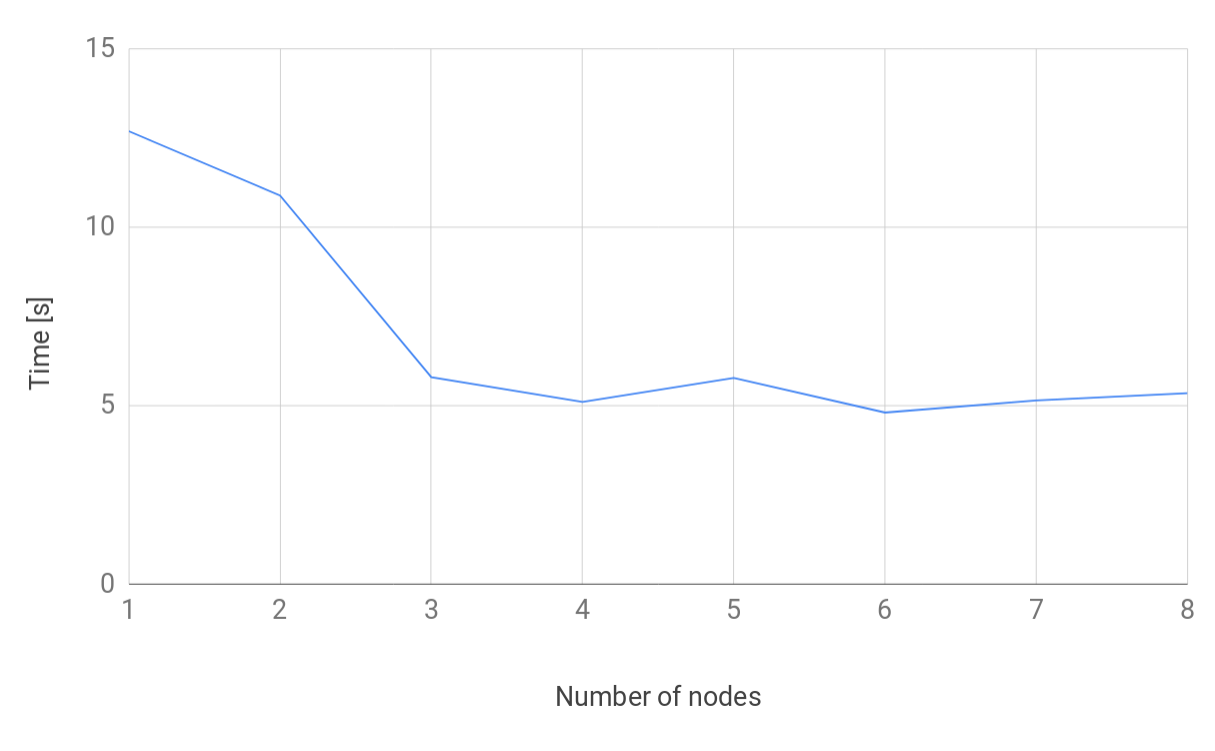
\includegraphics[width=0.8\textwidth]{thesis/figures/rf1.png}
            \caption{Time measurements for inserting 200,000 elements by one \Node with replication factor 1}
            \label{rf1}
        \end{figure}
    
        The second variant (Figure~\ref{rf3}) shows  a similar situation, but every key-value pair is replicated 3 times (the replication factor is equal to 3). A significant time overhead can be noticed due to used replication mechanism.
        If the network consists of only one \Node, then this \Node has to insert each element once. However, when the second \Node joins the system, every \Node has to insert every element twice -- in a local \PHT fragment and in a replicated \PHT fragment of the other \Node. The worst performance can be observed when the number of nodes is equal to the replication factor and thus every \Node has to insert each element three times.
        Afterwards the time needed for the data insertion is decreasing due to the work distribution. In the end, similarly to the previous test case, we reach a minimal time needed for one thread to process the data and to send proper messages. This behaviour proves the system scalability irrespective of the \textit{replication factor}.
        
        \begin{figure}[ht]
            \centering
            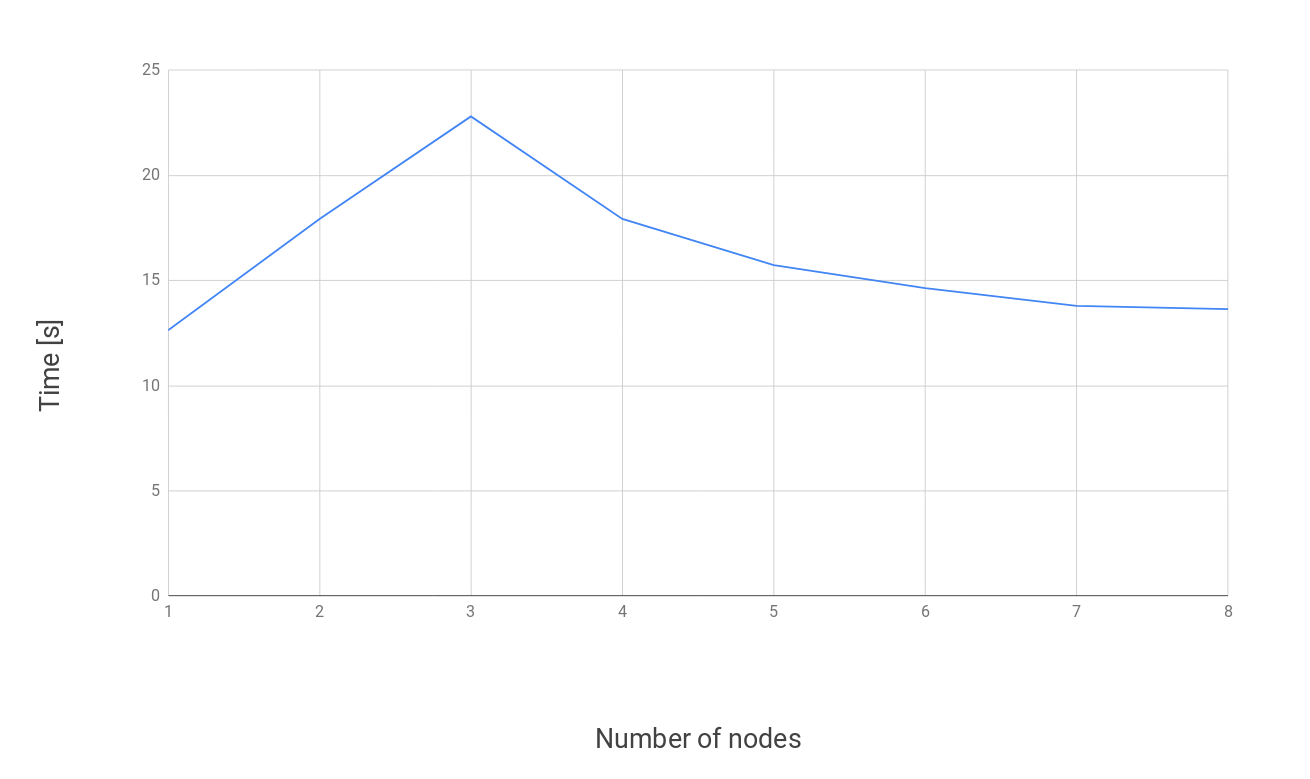
\includegraphics[width=0.8\textwidth]{thesis/figures/rf3.png}
            \caption{Time measurements for inserting 200,000 elements by one \Node with replication factor 3}
            \label{rf3}
        \end{figure}
        
        In the second test, whose results we give in Figure~\ref{mrf3}, we analysed the situation in which the inserted elements are equally distributed between the members of the cluster. The input data is processed by one thread on each \Node in opposition to the first test where only one thread on one \Node processed the input data. As a result, the insertion operation is completed in a shorter time than previously, even though replication factor is set to 3 and every element is inserted three times from the moment when
        number of \Nodes reaches 3.
    
    \begin{figure}[H]
        \centering
        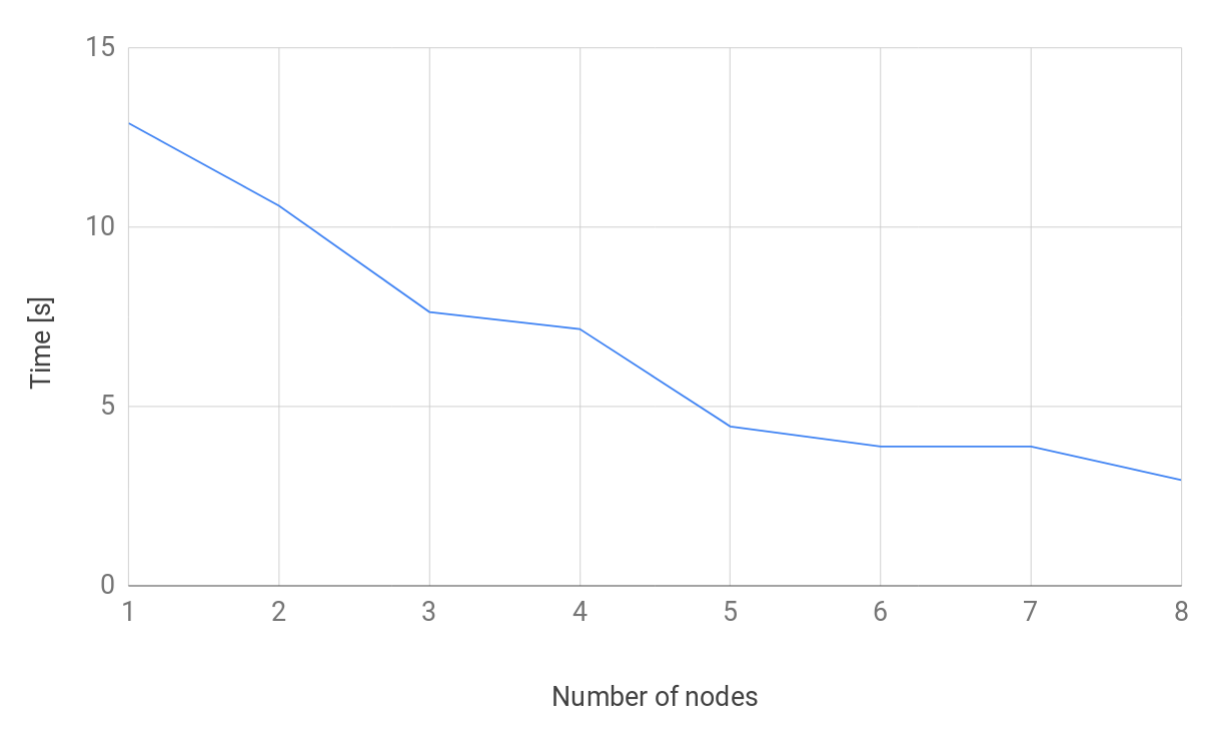
\includegraphics[width=0.8\textwidth]{thesis/figures/rf3MultipleInserts.png}
        \caption{Time measurements for multiple \Nodes inserting 200,000 elements altogether with replication factor 3}
        \label{mrf3}
    \end{figure}

\section{Conclusions}
    In this chapter we discussed \DHTS, a distributed system for the implemented \PHT class.
    
    We managed to develop a symmetrical and decentralised system in which each participant has the same set of responsibilities and there is no superior unit.
    It provides basic operations necessary to operate on \PHT such as \insertMethod, \getMethod and \removeMethod.
    We have also implemented consistent hashing and replication mechanisms which are common in these type of distributed applications.
    Extensive tests allowed us to ensure its correctness and uncover several bugs related to the communication process.

    The existing \DHTS implementation allowed us to test the scalability of \PHT in a distributed environment. The described system satisfies all the requirements of the project, but there is still room for improvement, especially in terms of efficient handling of failures.